\documentclass[journal, a4paper]{IEEEtran}
\usepackage{graphicx,url,amsmath, verbatim, float, moresize}   
\usepackage[brazil]{babel}
\usepackage[utf8]{inputenc, color}
\usepackage[T1]{fontenc}
\usepackage[compatibility,siunitx,  americanvoltages, americancurrents, americanresistors, europeaninductors, americanports,straightlabels, fetbodydiode, straightvoltages]{circuitikz}
\usepackage{tikz,amsmath, amssymb,bm,color,pgfkeys,siunitx,ifthen,ulem}
\usepackage{pgfplots}
\pgfplotsset{compat=1.14}
\usetikzlibrary{shapes,arrows}
\usetikzlibrary{circuits.ee.IEC}
\usetikzlibrary{arrows}
\usetikzlibrary{backgrounds,calc,positioning}
\ctikzset{tripoles/mos style/arrows}
\ctikzset{
	/tikz/circuitikz/quadpoles/coupler/width=1,%1.3
	/tikz/circuitikz/quadpoles/coupler/height=0.952,%1.3
	/tikz/circuitikz/quadpoles/coupler2/width=1,%1.3
	/tikz/circuitikz/quadpoles/coupler2/height=0.952,%1.3
	/tikz/circuitikz/quadpoles/transformer/width=1.425,%1.5
	/tikz/circuitikz/quadpoles/transformer/height=1.425,%1.5
	/tikz/circuitikz/quadpoles/transformer core/width=1.425,%1.5
	/tikz/circuitikz/quadpoles/transformer core/height=1.425,%1.5
	/tikz/circuitikz/quadpoles/gyrator/width=1.425,%1.5
	/tikz/circuitikz/quadpoles/gyrator/height=1.425,%1.5
	/tikz/circuitikz/monopoles/tlinestub/width=0.1875,%0.25 no effect!
	/tikz/circuitikz/tripoles/american and port/height=0.95,%.8
	/tikz/circuitikz/tripoles/american nand port/height=0.95,%.8
	/tikz/circuitikz/tripoles/american or port/height=0.95,%.8
	/tikz/circuitikz/tripoles/american nor port/height=0.95,%.8
	/tikz/circuitikz/tripoles/american xor port/height=0.95,%.8
	/tikz/circuitikz/tripoles/american xnor port/height=0.95,%.8
	/tikz/circuitikz/bipoles/tline/height=0.4,%0.3
%	/tikz/circuitikz/bipoles/tline/width=1.2,%0.8
	/tikz/circuitikz/bipoles/diode/height=0.375,%
	/tikz/circuitikz/bipoles/diode/width=0.375,%
	/tikz/circuitikz/bipoles/varcap/height=0.375,%
	/tikz/circuitikz/bipoles/varcap/width=0.375,%
	/tikz/circuitikz/tripoles/triac/height=1.05,%
	/tikz/circuitikz/tripoles/triac/width=0.952,%
	/tikz/circuitikz/tripoles/thyristor/height=1.05,%
	/tikz/circuitikz/tripoles/thyristor/width=0.952,%
	/tikz/circuitikz/tripoles/op amp/height=0.952,%
	/tikz/circuitikz/tripoles/op amp/width=1.2,%
	/tikz/circuitikz/tripoles/op amp/font=\footnotesize,
	/tikz/circuitikz/tripoles/gm amp/height=0.952,% 1.7
	/tikz/circuitikz/tripoles/gm amp/width=1.2,% 1.4
	%	/tikz/circuitikz/tripoles/gm amp/font=\footnotesize,
	/tikz/circuitikz/tripoles/plain amp/height=0.952,% 1.7
	/tikz/circuitikz/tripoles/plain amp/width=1.2,% 1.4
	/tikz/circuitikz/bipoles/resistor/voltage/straight label distance/.initial=.8,
	/tikz/circuitikz/bipoles/generic/voltage/straight label distance/.initial=.8,
	/tikz/circuitikz/bipoles/inductor/voltage/straight label distance/.initial=.8,
	/tikz/circuitikz/bipoles/fullgeneric/voltage/straight label distance/.initial=.8,
	/tikz/circuitikz/bipoles/capacitor/voltage/straight label distance/.initial=1.0,
	/tikz/circuitikz/bipoles/thickness=1.6,
}
\ctikzset{v/.append style={/tikz/european voltages}}

\definecolor{netlabelcolor}{rgb}{0, 0, 0.25}
\definecolor{lttotitextcolor}{rgb}{0, 0.4, 0.25}
\definecolor{lttotidrawcolor}{rgb}{0.6, 0.6, 0.6}
\definecolor{netcolor}{rgb}{0, 0, 0}

\pgfkeys{/lt2ti/netlabel/font/.initial= \small}
\pgfkeys{/lt2ti/text/font/.initial= \small}

\pgfkeys{/lt2ti/Net/.style= {netcolor}}
\tikzstyle{dashdotdotted}=[dash pattern=on 3pt off 2pt on \the\pgflinewidth off 2pt on \the\pgflinewidth off 2pt]

\pgfkeys{/lt2ti/VArrow/.style= {->,>=latex}}
\pgfkeys{/lt2ti/SArrow/.style= {->,>=angle 90}}

\begin{document}


	\title{Relatório 3 - Projeto de um Amplificador Emissor-Comum (EC)}
	\author{Arthur Pimentel e Matheus Farias

    }
	\maketitle
	\vspace{}
\section{Introdução}

    \tab A configuração emissor-comum (EC) possui duas características bastante atrativas, são elas: a) ganho de tensão da ordem de algumas centenas e b) resistência de entrada relativamente elevada. Tais características fazem desta configuração a mais empregada dos circuitos amplificadores de tensão com TBJ. Em amplificadores com múltiplos estágios, mais de um estágio EC pode ser usado para se obter o valor desejado do ganho de tensão total do amplificador. Há duas topologias clássicas para o amplificador EC: a) sem resistor de degeneração e b) com resistor de degeneração. O projetista deve escolher o circuito de polarização que melhor adequa-se as especificações do seu projeto, por exemplo, resistência de entrada, ganho de tensão, localização do ponto de operação, etc.

\section{Projeto}
	
    \tab Na disciplina de Eletrônica 1 foram vistos quatro tipos de polarização de amplificadores. Estes são: Polarização por divisão de tensão, Polarização com duas fontes simétricas, Polarização com Resistor de realimentação Base-Coletor e Polarização usando uma fonte de corrente constante.
    
    \tab Ficou a critério do projetista escolher o tipo da polarização do amplificador usado.
    
    \tab No design do amplificador desejado, inicialmente, escolheu-se o modo de polarização por divisão de tensão sem resistor de degeneração para pequenos sinais.  
    
    \tab Observa-se, na Figura \ref{EM sem re}, a configuração idealizada para o projeto.
    
    \makeatletter

%% bandstop filter (adapted from highpass)
\pgfcircdeclarebipole{}{\ctikzvalof{bipoles/highpass/width}}{*bandstop}{\ctikzvalof{bipoles/highpass/width}}{\ctikzvalof{bipoles/highpass/width}}{
	\pgf@circ@res@step = \ctikzvalof{bipoles/highpass/width}\pgf@circ@Rlen
	\divide \pgf@circ@res@step by 2
	
	\pgfpathmoveto{\pgfpoint{\pgf@circ@res@left}{\pgf@circ@res@zero}}
	\pgf@circ@res@other = \pgf@circ@res@left
	\advance\pgf@circ@res@other by \pgf@circ@res@step 
	
	\ifpgf@circuit@dashed
	\pgfsetdash{{0.1cm}{0.1cm}}{0cm} 
	\fi	
	
	% draw outer box
	\pgfsetlinewidth{\pgfkeysvalueof{/tikz/circuitikz/bipoles/thickness}\pgfstartlinewidth}
	\pgfpathrectanglecorners{\pgfpoint{\pgf@circ@res@left}{\pgf@circ@res@up}}{\pgfpoint{\pgf@circ@res@right}{\pgf@circ@res@down}}
	\pgfusepath{draw}
	
	\ifpgf@circuit@inputarrow
	{
		\advance \pgf@circ@res@left by -.5\pgfkeysvalueof{/tikz/circuitikz/bipoles/thickness}\pgfstartlinewidth
		\pgftransformshift{\pgfpoint{\pgf@circ@res@left}{0pt}}
		\pgfnode{inputarrow}{tip}{}{pgf@inputarrow}{\pgfusepath{fill}}
	}
	\fi
	
	% rotate inner symbol
	\def\pgfcircmathresult{\expandafter\pgf@circ@stripdecimals\pgf@circ@direction\pgf@nil}
	\ifnum \pgfcircmathresult > 45 \ifnum \pgfcircmathresult < 135
	\pgftransformrotate{270}
	\fi\fi
	\ifnum \pgfcircmathresult > 134 \ifnum \pgfcircmathresult < 225  % 134 degree, because >= 135 is not possible
	\pgftransformrotate{180}
	\fi\fi
	\ifnum \pgfcircmathresult > 224 \ifnum \pgfcircmathresult < 315
	\pgftransformrotate{90}
	\fi\fi
	
	% draw inner symbol
	\pgfsetdash{}{0pt}	% always draw solid line for inner symbol
	\pgfsetarrows{-} %never draw arrows
	\pgfsetlinewidth{\pgfstartlinewidth}
	\pgfpathmoveto{\pgfpoint{-0.5\pgf@circ@res@step}{0.5\pgf@circ@res@step}}
	\pgfpathsine{\pgfpoint{.25\pgf@circ@res@step}{.25\pgf@circ@res@step}}
	\pgfpathcosine{\pgfpoint{.25\pgf@circ@res@step}{-.25\pgf@circ@res@step}}
	\pgfpathsine{\pgfpoint{.25\pgf@circ@res@step}{-.25\pgf@circ@res@step}}
	\pgfpathcosine{\pgfpoint{.25\pgf@circ@res@step}{.25\pgf@circ@res@step}}
	\pgfusepath{draw}
	
	\pgfpathmoveto{\pgfpoint{-0.5\pgf@circ@res@step}{0}}
	\pgfpathsine{\pgfpoint{.25\pgf@circ@res@step}{.25\pgf@circ@res@step}}
	\pgfpathcosine{\pgfpoint{.25\pgf@circ@res@step}{-.25\pgf@circ@res@step}}
	\pgfpathsine{\pgfpoint{.25\pgf@circ@res@step}{-.25\pgf@circ@res@step}}
	\pgfpathcosine{\pgfpoint{.25\pgf@circ@res@step}{.25\pgf@circ@res@step}}
	\pgfusepath{draw}
	\pgfpathmoveto{\pgfpoint{-0.15\pgf@circ@res@step}{-0.15\pgf@circ@res@step}}
	\pgfpathlineto{\pgfpoint{0.15\pgf@circ@res@step}{0.15\pgf@circ@res@step}}
	\pgfusepath{draw}
	
	\pgfpathmoveto{\pgfpoint{-0.5\pgf@circ@res@step}{-0.5\pgf@circ@res@step}}
	\pgfpathsine{\pgfpoint{.25\pgf@circ@res@step}{.25\pgf@circ@res@step}}
	\pgfpathcosine{\pgfpoint{.25\pgf@circ@res@step}{-.25\pgf@circ@res@step}}
	\pgfpathsine{\pgfpoint{.25\pgf@circ@res@step}{-.25\pgf@circ@res@step}}
	\pgfpathcosine{\pgfpoint{.25\pgf@circ@res@step}{.25\pgf@circ@res@step}}
	\pgfusepath{draw}
	%	\pgfpathmoveto{\pgfpoint{-0.15\pgf@circ@res@step}{-0.65\pgf@circ@res@step}}
	%	\pgfpathlineto{\pgfpoint{0.15\pgf@circ@res@step}{-0.35\pgf@circ@res@step}}
	%	\pgfusepath{draw}
}

\tikzset{
	*bandstop/.style={\circuitikzbasekey, /tikz/to path=\pgf@circ@*bandstop@path},
}
\def\pgf@circ@*bandstop@path#1{\pgf@circ@bipole@path{*bandstop}{#1}}




\makeatother
    
  %    \tab  {\color{red}MOSTRAR DESENHO DO CIRCUITO}
    
	\begin{figure}[H]
	
	    \hspace{-0.8 cm}	
    	\begin{tikzpicture}[circuit ee IEC, scale=0.5666666667,line width=.5pt]% default: 0.4
	%\tikzstyle{every node}=[font=\small];%
	%\node [draw] at (0.0,0.0) {\pgfkeysvalueof{/tikz/circuitikz/tripoles/op amp/font}};
%\draw [/lt2ti/Net](22.0,22.5)to[*short,*-, color=netcolor] (22.0,22.5);% wire w3_w6 start
%\draw [/lt2ti/Net](15.5,21.0)to[*short,-, color=netcolor] (15.5,21.0);% wire w3_w6 end
%\draw [/lt2ti/Net](22.0,22.5) --  (15.5,22.5) -- (15.5,21.0); % wire w3_w6 polyline 
%\draw [/lt2ti/Net](27.0,22.0)to[*short,-, color=netcolor] (27.0,22.0);% wire w4_w5 start
%\draw [/lt2ti/Net](22.0,22.5)to[*short,-*, color=netcolor] (22.0,22.5);% wire w4_w5 end
%\draw [/lt2ti/Net](27.0,22.0) --  (27.0,22.5) -- (22.0,22.5); % wire w4_w5 polyline 
%\draw [/lt2ti/Net](22.0,21.0)to[*short,-*, color=netcolor] (22.0,22.5);% wire w7
\draw [/lt2ti/Net](27.0,18.5)to[*short,*-, color=netcolor] (27.0,19.0);% wire w8
\draw [/lt2ti/Net](28.0,18.5)to[*short,-*, color=netcolor] (27.0,18.5);% wire w9
%\draw [/lt2ti/Net](15.5,17.5)to[*short,-, color=netcolor] (15.5,18.5);% wire w11
\draw [/lt2ti/Net](31.5,17.5)to[*short,-, color=netcolor] (31.5,17.5);% wire w10_w12 start
\draw [/lt2ti/Net](30.0,18.5)to[*short,-, color=netcolor] (30.0,18.5);% wire w10_w12 end
\draw [/lt2ti/Net](31.5,17.5) --  (31.5,18.5) -- (30.0,18.5); % wire w10_w12 polyline 
\draw [/lt2ti/Net](19.5,17.0)to[*short,-, color=netcolor] (19.5,17.0);% wire w13_w18 start
\draw [/lt2ti/Net](18.0,16.0)to[*short,-, color=netcolor] (18.0,16.0);% wire w13_w18 end
\draw [/lt2ti/Net](19.5,17.0) --  (18.0,17.0) -- (18.0,16.0); % wire w13_w18 polyline 
\draw [/lt2ti/Net](22.0,17.0)to[*short,*-, color=netcolor] (22.0,18);% wire w14
\draw [/lt2ti/Net](22.0,17.0)to[*short,*-, color=netcolor] (21.5,17.0);% wire w15
\draw [/lt2ti/Net](25.0,17.0)to[*short,-, color=netcolor] (25.0,17.0);% wire w16_w17 start
\draw [/lt2ti/Net](22.0,17.0)to[*short,-*, color=netcolor] (22.0,17.0);% wire w16_w17 end
\draw [/lt2ti/Net](25.0,17.0) --  (24.0,17.0) -- (22.0,17.0); % wire w16_w17 polyline 
\draw [/lt2ti/Net](22.0,16.0)to[*short,-*, color=netcolor] (22.0,17.0);% wire w19
\draw [/lt2ti/Net](27.0,15.0)to[*short,*-, color=netcolor] (27.0,15.5);% wire w20
\draw [/lt2ti/Net](27.0,14.5)to[*short,-*, color=netcolor] (27.0,15.0);% wire w22
\draw [/lt2ti/Net](29.5,14.0)to[*short,-, color=netcolor] (29.5,14.0);% wire w21_w23 start
\draw [/lt2ti/Net](27.0,15.0)to[*short,-*, color=netcolor] (27.0,15.0);% wire w21_w23 end
\draw [/lt2ti/Net](29.5,14.0) --  (29.5,15.0) -- (27.0,15.0); % wire w21_w23 polyline 
\draw [/lt2ti/Net](31.5,13.5)to[*short,-, color=netcolor] (31.5,15.0);% wire w24
\draw [/lt2ti/Net](22.0,11.5)to[*short,*-, color=netcolor] (22.0,13.5);% wire w26
\draw [/lt2ti/Net](22.0,11.5)to[*short,*-, color=netcolor] (22.0,11.5);% wire w25_w27 start
\draw [/lt2ti/Net](18.0,13.5)to[*short,-, color=netcolor] (18.0,13.5);% wire w25_w27 end
\draw [/lt2ti/Net](22.0,11.5) --  (18.0,11.5) -- (18.0,13.5); % wire w25_w27 polyline 
\draw [/lt2ti/Net](24.0,11.5)to[*short,*-*, color=netcolor] (22.0,11.5);% wire w28
\draw [/lt2ti/Net](27.0,11.5)to[*short,*-, color=netcolor] (27.0,12.0);% wire w29
\draw [/lt2ti/Net](27.0,11.5)to[*short,*-*, color=netcolor] (24.0,11.5);% wire w30
\draw [/lt2ti/Net](29.5,12.0)to[*short,-, color=netcolor] (29.5,12.0);% wire w31_w32 start
\draw [/lt2ti/Net](27.0,11.5)to[*short,-*, color=netcolor] (27.0,11.5);% wire w31_w32 end
\draw [/lt2ti/Net](29.5,12.0) --  (29.5,11.5) -- (27.0,11.5); % wire w31_w32 polyline 
\draw [/lt2ti/Net](24.0,10.0)to[*short,-*, color=netcolor] (24.0,11.5);% wire w33
\draw [/lt2ti/Net](22.0,20.5)to[,-*, color=netcolor] (22.0,21.5);% wire teste
 %\draw (15.5, 17.5) node[ground, xscale=2, yscale=2, rotate=270, ] (undefined) {};%  (undefined)++(0.0,0.0) node {undefined }; % component "circuiTikz\\gnd" "undefined" 
 \draw (24.0, 10.0) node[ground, xscale=2, yscale=2, rotate=270, ] (undefined) {};%  (undefined)++(0.0,0.0) node {undefined }; % component "circuiTikz\\gnd" "undefined" 
 \draw (31.5, 13.5) node[ground, xscale=2, yscale=2, rotate=270, ] (undefined) {};%  (undefined)++(0.0,0.0) node {undefined }; % component "circuiTikz\\gnd" "undefined" 
  \draw (22.0, 20.5) to[*resistor, l^=R\textsubscript{1},  -, ] (22.0,18){}; %\node [] at (21.5,21.5) {x}; % component "res" "R9" 
  \draw  --++(22,21.5) node[vcc]{+\,\textnormal{V\textsubscript{CC}}}{};% to (22,20.5){};
  \draw (22.0, 16.0) to[*resistor, l^=R\textsubscript{2}, , -, ] (22.0,13.5){}; %\node [] at (21.5,16.5) {x}; % component "res" "R10" 
  \draw (27.0, 21.5) to[*resistor, l^=R\textsubscript{C},  -, ] (27.0,19.0){}; %\node [] at (26.5,22.5) {x}; % component "res" "R11" 
  \draw  --++(27,21.5) node[vcc]{+\,\textnormal{V\textsubscript{CC}}} to (27,21.5){};
  \draw (27.0, 14.5) to[*resistor, a_=R\textsubscript{E}, -, ] (27.0,12.0){}; %\node [] at (26.5,15.0) {x}; % component "res" "R12" 
 \draw (27.0, 17.0) node[npn, nobodydiode, , rotate=0, ] (Q3) {}   (Q3)++(1.0,1) ; % component "npn" "Q3" 
 \draw (25.0, 17.0) to [*short, -] (Q3.B); \draw (27.0, 15.5) to [*short, -] (Q3.E); \draw (27.0, 18.5) to [*short, -] (Q3.C);% extend wires to the connection points   % component "npn" "Q3" 
 % \draw (15.5, 21.0) to[*V, l_=V\textsubscript{CC}, , -, ] (15.5,18.5){}; % component "voltage" "V5" 
  \draw (21.5, 17.0) to[*capacitor, l^=C,  -, ] (19.5,17.0){}; % component "cap" "C5" 
  %\node [] at (21.5,17.5) {x}; % component "cap" "C5" 
  \draw (30.0, 18.5) to[*capacitor, l^=C,  -, ] (28.0,18.5){}; % component "cap" "C6" 
  %\node [] at (30.0,19.0) {x}; % component "cap" "C6" 
  \draw (18.0, 16.0) to[*V, l_=V\textsubscript{sig},, -, ] (18.0,13.5){}; % component "voltage" "V3" 
  \draw (29.5, 14.0) to[*capacitor, a_=C,  -, ] (29.5,12.0){}; % component "cap" "C3" 
  %\node [] at (29.0,14.0) {x}; % component "cap" "C3" 
  \draw (31.5, 17.5) to[*resistor, l^=R\textsubscript{L},  -, ] (31.5,15.0){}; %\node [] at (31.0,18.0) {x}; % component "res" "R6" 
  \node (Vo) [] at (31.5,18.5) {};% label mark % label "" "Vo" lbl37 
%  \node (Votxt) [ netlabelcolor, above= -0.24cm of Vo] {{\pgfkeysvalueof{/lt2ti/netlabel/font}Vo}}; % label "" "Vo" lbl37 
  \node (Vi) [] at (24.0,17.0) {};% label mark % label "" "Vi" lbl38 
%  \node (Vitxt) [ netlabelcolor, above= -0.24cm of Vi] {{\pgfkeysvalueof{/lt2ti/netlabel/font}Vi}}; % label "" "Vi" lbl38 
  \node (Vsig) [] at (18.0,17.0) {};% label mark % label "" "Vsig" lbl39 
%  \node (Vsigtxt) [ netlabelcolor, above= -0.24cm of Vsig] {{\pgfkeysvalueof{/lt2ti/netlabel/font}Vsig}}; % label "" "Vsig" lbl39 
  \node (lbl83) [] at (17.0,10.25) {};% text mark % text "" ".tran 1ms lbl83 " 
  %\node (lbl83txt) [ lttotitextcolor, right= -0.25cm of lbl83, scale=0.5*2.0] {{\pgfkeysvalueof{/lt2ti/text/font}.tran 1ms}}; % text "" ".tran 1ms lbl83 " 

	\end{tikzpicture}
	
	
	
	
	
	
	
	
	
	
	
	
	
	
	
	
	
	
	
	
	
	
	
	
	
	
	
	
	
	
	
	
	
	
	
	
	
	
	
	
	
	
	
	
	
	
	
	
	
	
	
%%%%%%%%%%%%%%%%%%%%%%%%%%%%%%%%%%%%%%%%%%%%%%%%%%%%%%%%%%%%%%%%%%%%%%%%%%%%%%% VERSÃO ANTIGA%%%%%%%%%%%%%%%%%%%%%%%%%%%%%%% %%%%%%%%%%%%%%%%%%%%%%%%%%%%%%%%%%%%%%%%%%%%%%%%%%
\begin{comment}
\begin{tikzpicture}[circuit ee IEC, scale=0.4666666667,line width=.5pt]
           % \hspace{-0.8 cm}
        	% default: 0.4
        	%\tikzstyle{every node}=[font=\small];%
        	%\node [draw] at (0.0,0.0) {\pgfkeysvalueof{/tikz/circuitikz/tripoles/op amp/font}};
        \draw [/lt2ti/Net](22.0,22.5)to[*short,*-, color=netcolor] (22.0,22.5);% wire w3_w6 start
        \draw [/lt2ti/Net](15.5,21.0)to[*short,-, color=netcolor] (15.5,21.0);% wire w3_w6 end
        \draw [/lt2ti/Net](22.0,22.5) --  (15.5,22.5) -- (15.5,21.0); % wire w3_w6 polyline 
        \draw [/lt2ti/Net](27.0,22.0)to[*short,-, color=netcolor] (27.0,22.0);% wire w4_w5 start
        \draw [/lt2ti/Net](22.0,22.5)to[*short,-*, color=netcolor] (22.0,22.5);% wire w4_w5 end
        \draw [/lt2ti/Net](27.0,22.0) --  (27.0,22.5) -- (22.0,22.5); % wire w4_w5 polyline 
        \draw [/lt2ti/Net](22.0,21.0)to[*short,-*, color=netcolor] (22.0,22.5);% wire w7
        \draw [/lt2ti/Net](27.0,18.5)to[*short,*-, color=netcolor] (27.0,19.5);% wire w8
        \draw [/lt2ti/Net](28.0,18.5)to[*short,-*, color=netcolor] (27.0,18.5);% wire w9
        \draw [/lt2ti/Net](15.5,17.5)to[*short,-, color=netcolor] (15.5,18.5);% wire w11
        \draw [/lt2ti/Net](31.5,17.5)to[*short,-, color=netcolor] (31.5,17.5);% wire w10_w12 start
        \draw [/lt2ti/Net](30.0,18.5)to[*short,-, color=netcolor] (30.0,18.5);% wire w10_w12 end
        \draw [/lt2ti/Net](31.5,17.5) --  (31.5,18.5) -- (30.0,18.5); % wire w10_w12 polyline 
        \draw [/lt2ti/Net](19.5,17.0)to[*short,-, color=netcolor] (19.5,17.0);% wire w13_w18 start
        \draw [/lt2ti/Net](18.0,16.0)to[*short,-, color=netcolor] (18.0,16.0);% wire w13_w18 end
        \draw [/lt2ti/Net](19.5,17.0) --  (18.0,17.0) -- (18.0,16.0); % wire w13_w18 polyline 
        \draw [/lt2ti/Net](22.0,17.0)to[*short,*-, color=netcolor] (22.0,18.5);% wire w14
        \draw [/lt2ti/Net](22.0,17.0)to[*short,*-, color=netcolor] (21.5,17.0);% wire w15
        \draw [/lt2ti/Net](25.0,17.0)to[*short,-, color=netcolor] (25.0,17.0);% wire w16_w17 start
        \draw [/lt2ti/Net](22.0,17.0)to[*short,-*, color=netcolor] (22.0,17.0);% wire w16_w17 end
        \draw [/lt2ti/Net](25.0,17.0) --  (24.0,17.0) -- (22.0,17.0); % wire w16_w17 polyline 
        \draw [/lt2ti/Net](22.0,16.0)to[*short,-*, color=netcolor] (22.0,17.0);% wire w19
        \draw [/lt2ti/Net](27.0,15.0)to[*short,*-, color=netcolor] (27.0,15.5);% wire w20
        \draw [/lt2ti/Net](27.0,14.5)to[*short,-*, color=netcolor] (27.0,15.0);% wire w22
        \draw [/lt2ti/Net](29.5,14.0)to[*short,-, color=netcolor] (29.5,14.0);% wire w21_w23 start
        \draw [/lt2ti/Net](27.0,15.0)to[*short,-*, color=netcolor] (27.0,15.0);% wire w21_w23 end
        \draw [/lt2ti/Net](29.5,14.0) --  (29.5,15.0) -- (27.0,15.0); % wire w21_w23 polyline 
        \draw [/lt2ti/Net](31.5,13.5)to[*short,-, color=netcolor] (31.5,15.0);% wire w24
        \draw [/lt2ti/Net](22.0,11.5)to[*short,*-, color=netcolor] (22.0,13.5);% wire w26
        \draw [/lt2ti/Net](22.0,11.5)to[*short,*-, color=netcolor] (22.0,11.5);% wire w25_w27 start
        \draw [/lt2ti/Net](18.0,13.5)to[*short,-, color=netcolor] (18.0,13.5);% wire w25_w27 end
        \draw [/lt2ti/Net](22.0,11.5) --  (18.0,11.5) -- (18.0,13.5); % wire w25_w27 polyline 
        \draw [/lt2ti/Net](24.0,11.5)to[*short,*-*, color=netcolor] (22.0,11.5);% wire w28
        \draw [/lt2ti/Net](27.0,11.5)to[*short,*-, color=netcolor] (27.0,12.0);% wire w29
        \draw [/lt2ti/Net](27.0,11.5)to[*short,*-*, color=netcolor] (24.0,11.5);% wire w30
        \draw [/lt2ti/Net](29.5,12.0)to[*short,-, color=netcolor] (29.5,12.0);% wire w31_w32 start
        \draw [/lt2ti/Net](27.0,11.5)to[*short,-*, color=netcolor] (27.0,11.5);% wire w31_w32 end
        \draw [/lt2ti/Net](29.5,12.0) --  (29.5,11.5) -- (27.0,11.5); % wire w31_w32 polyline 
        \draw [/lt2ti/Net](24.0,10.0)to[*short,-*, color=netcolor] (24.0,11.5);% wire w33
        \draw [/lt2ti/Net](22.0,20.5)to[,-*, color=netcolor] (22.0,21.5);% wire teste
         \draw (15.5, 17.5) node[ground, xscale=2, yscale=2, rotate=270, ] (undefined) {};%  (undefined)++(0.0,0.0) node {undefined }; % component "circuiTikz\\gnd" "undefined" 
         \draw (24.0, 10.0) node[ground, xscale=2, yscale=2, rotate=270, ] (undefined) {};%  (undefined)++(0.0,0.0) node {undefined }; % component "circuiTikz\\gnd" "undefined" 
         \draw (31.5, 13.5) node[ground, xscale=2, yscale=2, rotate=270, ] (undefined) {};%  (undefined)++(0.0,0.0) node {undefined }; % component "circuiTikz\\gnd" "undefined" 
          \draw (22.0, 21.0) to[*resistor, l^=R\textsubscript{1},  -, ] (22.0,18.5){}; %\node [] at (21.5,21.5) {x}; % component "res" "R9" 
          \draw (22.0, 16.0) to[*resistor, l^=R\textsubscript{2}, , -, ] (22.0,13.5){}; %\node [] at (21.5,16.5) {x}; % component "res" "R10" 
          \draw (27.0, 22.0) to[*resistor, l^=R\textsubscript{C},  -, ] (27.0,19.5){}; %\node [] at (26.5,22.5) {x}; % component "res" "R11" 
          \draw (27.0, 14.5) to[*resistor, a_=R\textsubscript{E}, -, ] (27.0,12.0){}; %\node [] at (26.5,15.0) {x}; % component "res" "R12" 
         \draw (27.0, 17.0) node[npn, nobodydiode, , rotate=0, ] (Q3) {}   (Q3)++(1.0,1) ; % component "npn" "Q3" 
         \draw (25.0, 17.0) to [*short, -] (Q3.B); \draw (27.0, 15.5) to [*short, -] (Q3.E); \draw (27.0, 18.5) to [*short, -] (Q3.C);% extend wires to the connection points   % component "npn" "Q3" 
          \draw (15.5, 21.0) to[*V, l_=V\textsubscript{CC}, , -, ] (15.5,18.5){}; % component "voltage" "V5" 
          \draw (21.5, 17.0) to[*capacitor, l^=C,  -, ] (19.5,17.0){}; % component "cap" "C5" 
          %\node [] at (21.5,17.5) {x}; % component "cap" "C5" 
          \draw (30.0, 18.5) to[*capacitor, l^=C,  -, ] (28.0,18.5){}; % component "cap" "C6" 
          %\node [] at (30.0,19.0) {x}; % component "cap" "C6" 
          \draw (18.0, 16.0) to[*V, l_=V\textsubscript{sig}, , -, ] (18.0,13.5){}; % component "voltage" "V3" 
          \draw (29.5, 14.0) to[*capacitor, a_=C,  -, ] (29.5,12.0){}; % component "cap" "C3" 
          %\node [] at (29.0,14.0) {x}; % component "cap" "C3" 
          \draw (31.5, 17.5) to[*resistor, l^=R\textsubscript{L},  -, ] (31.5,15.0){}; %\node [] at (31.0,18.0) {x}; % component "res" "R6" 
          \node (Vo) [] at (31.5,18.5) {};% label mark % label "" "Vo" lbl37 
        %  \node (Votxt) [ netlabelcolor, above= -0.24cm of Vo] {{\pgfkeysvalueof{/lt2ti/netlabel/font}Vo}}; % label "" "Vo" lbl37 
          \node (Vi) [] at (24.0,17.0) {};% label mark % label "" "Vi" lbl38 
        %  \node (Vitxt) [ netlabelcolor, above= -0.24cm of Vi] {{\pgfkeysvalueof{/lt2ti/netlabel/font}Vi}}; % label "" "Vi" lbl38 
          \node (Vsig) [] at (18.0,17.0) {};% label mark % label "" "Vsig" lbl39 
        %  \node (Vsigtxt) [ netlabelcolor, above= -0.24cm of Vsig] {{\pgfkeysvalueof{/lt2ti/netlabel/font}Vsig}}; % label "" "Vsig" lbl39 
          \node (lbl83) [] at (17.0,10.25) {};% text mark % text "" ".tran 1ms lbl83 " 
          %\node (lbl83txt) [ lttotitextcolor, right= -0.25cm of lbl83, scale=0.5*2.0] {{\pgfkeysvalueof{/lt2ti/text/font}.tran 1ms}}; % text "" ".tran 1ms lbl83 " 

	\end{tikzpicture}
\end{comment}
    	
	    \caption{Amplificador Emissor-Comum sem resistor de degeneração.}
	    \label{EM sem re}
    \end{figure}
	
    \tab A partir da configuração escolhida, determina-se, arbitrariamente, alguns valores iniciais do amplificador. Lembrando das limitação impostas sobre o projetista. Estas são:
         \begin{itemize}
                \item $A_v = -100 \: $V/V.
                
                \item $R_L = 1 \: k\Omega$.
                
                \item $v_{sig}$ senoidal com valor de pico igual a 20 mV e frequência igual a 8 kHz.
                
                \item  Fonte de alimentação independente $0$ V $\leq \: V_{CC} \: \leq \: 20$ V ou Fonte de alimentação simétrica $0$ V $ \leq |V_{CC}|, \: |V_{EE}| \leq 20 \: $ V.
            \end{itemize}
    \tab Escolheu-se: 
    
         \begin{itemize}
                \item $V_{CC} = 10 \:$V .
                
                \item $V_{E} = 1 \:$V.
                
                \item $V_C = \frac{V_{CC}}{2}$.
                
                \item $C = \SI{470}{\micro\farad}$  
                
            \end{itemize}
       
    \tab A partir da análise c.a dos amplificador, usando o modelo T, tem-se que:
     
       $$     A_v = \frac{-\alpha(R_C//R_L)}{r_e} = -100 $$
      
    \tab Assim, 
     
       $$     r_e = \frac{\alpha(R_C//R_L)}{100} = \frac{0,025}{I_E} $$
      
      $$ \frac{1000R_C}{R_C + 1000} = \frac{2,5}{I_C} $$
      
      $$ 1000 R_C I_C = 2,5R_C + 2500 $$
      
    \tab Escolhe-se $R_C = \SI{1}{\kilo\ohm}$ e, consequentemente, $I_C =\SI{5}{\milli\ampere}$.
    
    \tab Assim, $I_E = \frac{I_C}{\alpha} =\SI{5,05}{\milli\ampere}$ e $R_E  = \frac{1}{5,05 \times 10^{-3}} = 198 \: \Omega$
    
    \tab Finalmente, seleciona-se $R_1$ e $R_2$ de forma a satisfazer as condições estabelecidas. Escolhe-se que as correntes que passam por $R_1$ e $R_2$ são $11 I_B$ e $10 I_B$, respectivamente. Resultando em $R_1 = \SI{15,1}{\kilo\ohm}$ e $R_2 = \SI{3,4}{\kilo\ohm}$.
    
    \tab Verifica-se na análise c.c que o amplificador permanece no modo ativo direto.

\section{Simulação}
    \tab Com o auxílio do \textit{Software} LT{\ssmall SPICE} IV, simulou-se o circuito descrito anteriormente e obteve-se o valor de $A_v$ do amplificador.
    
    \tab Observa-se o circuito na Figura \ref{circuit ideal com distorção}.
         \begin{figure}[H]
    		\begin{center}
    		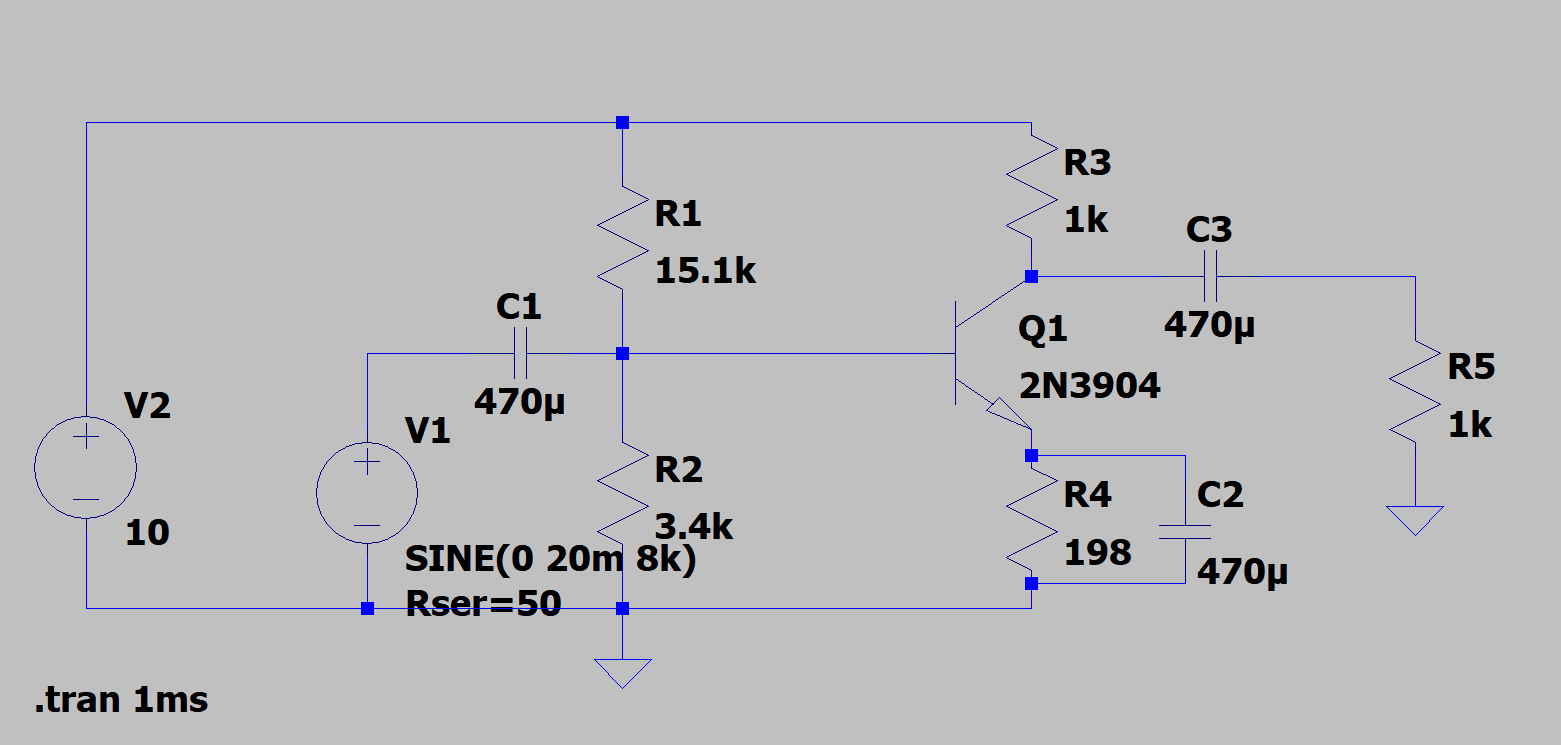
\includegraphics[width=\columnwidth]{circuito_ideal_distorcao.PNG}
    		\caption{Simulaçao do amplificador Emissor-Comum sem resistor de degeneração.}
    		\label{circuit ideal com distorção}
    		\end{center}
    	\end{figure}
    	
    \tab Em seguida, com o auxílio da ferramenta \textit{Cursor}, verificou-se o ganho $A_v$ do amplificador. Em que, $A_v = \frac{V_o}{V_i} = \frac{3,822}{37,91 \times 10^{-3}} = 100,8$ V/V
    
    \tab Observa-se as formas de onda de $V_o$ e $V_i$ no modo \textit{Osciloscópio} do  LT{\ssmall SPICE} na Figura \ref{osciloscopio ideal com distorção}.
        \begin{figure}[H]
    		\begin{center}
    		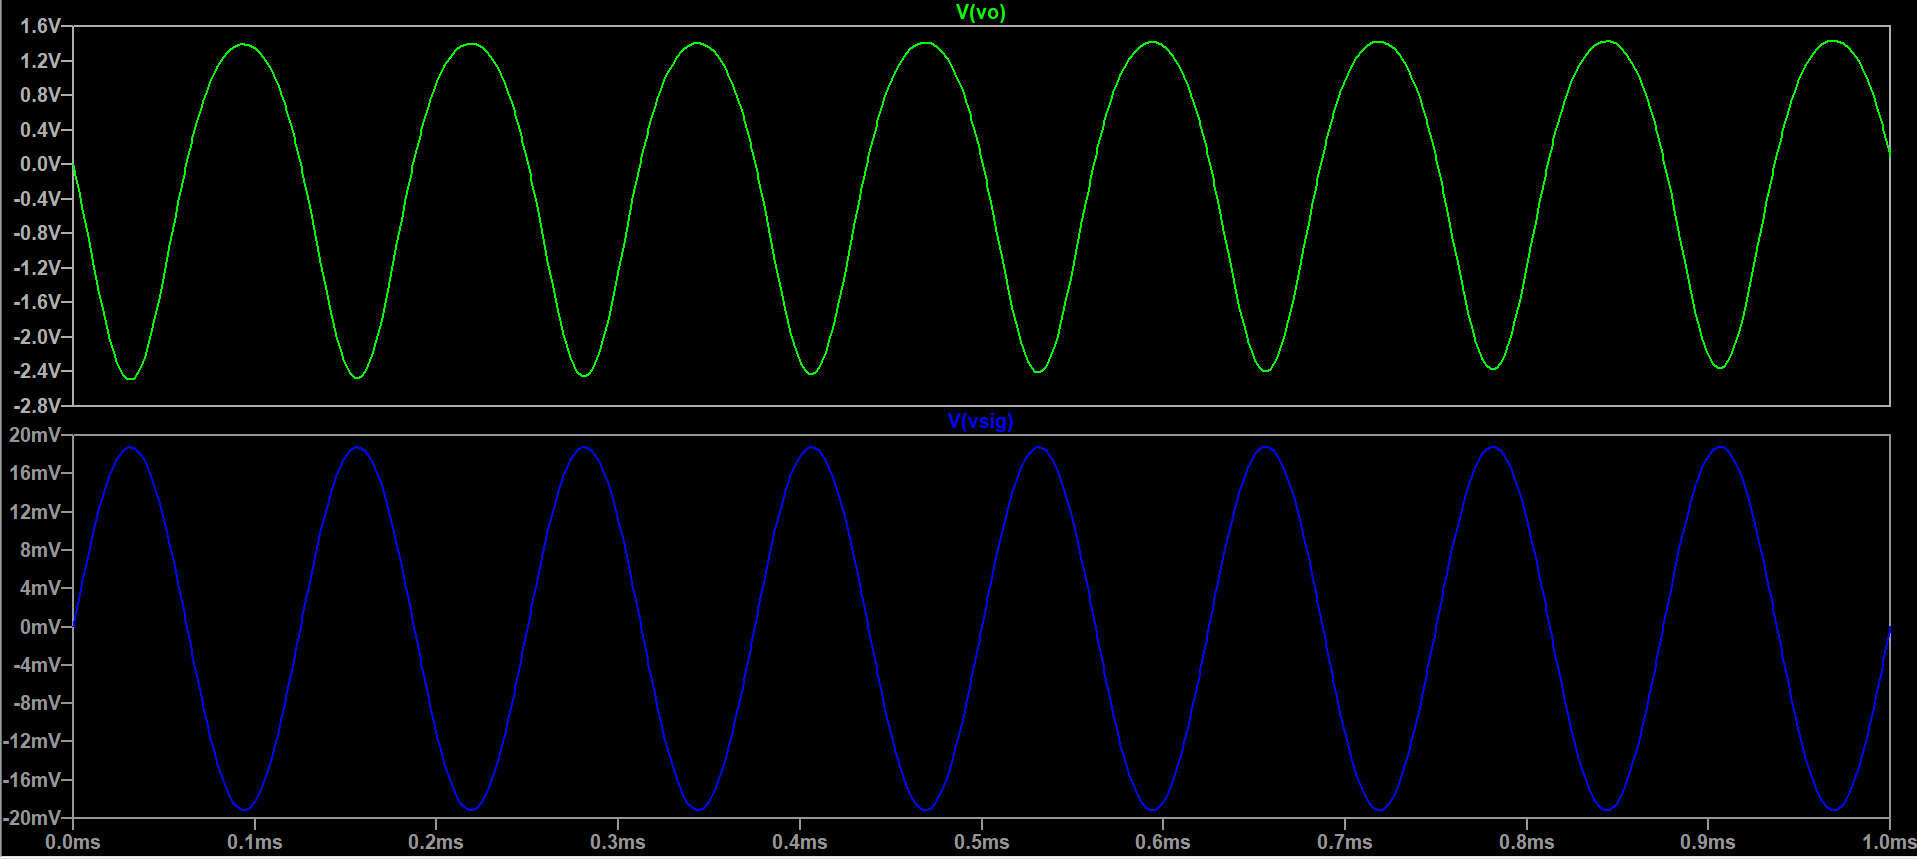
\includegraphics[width=\columnwidth]{Av_ideal_distorcao2.PNG}
    		\caption{Formas de onda de $V_o$ e $V_i$ do circuito da Figura \ref{circuit ideal com distorção}.}
    		\label{osciloscopio ideal com distorção}
    		\end{center}
    	\end{figure}
        
\section{Experimento}
    \tab Na etapa experimental, foi necessário adaptar os resistores calculados para resistores usuais. Felizmente, o amplificador foi projetado com esse passo em mente e encontrou-se resistores com valores reais próximos dos valores teóricos ideais. Mesmo assim, após a utilização dos resistores reais, percebeu-se uma redução no ganho. Assim, foi necessitou-se realizar um ajuste na fonte de tensão de 10 V para 11 V para manter o ganho $A_v = -100 \:$V/V.
    
    \tab Observa-se, na Figura \ref{osciloscopio lab com distorção}, a imagem da tela do osciloscópio medindo $V_i$ (em amarelo) e $V_o$ (em verde). Nota-se que $A_v = \frac{3,754}{37,2 \times 10^{-3}} = 100,9 \:$V/V.
        \begin{figure}[H]
    		\begin{center}
    		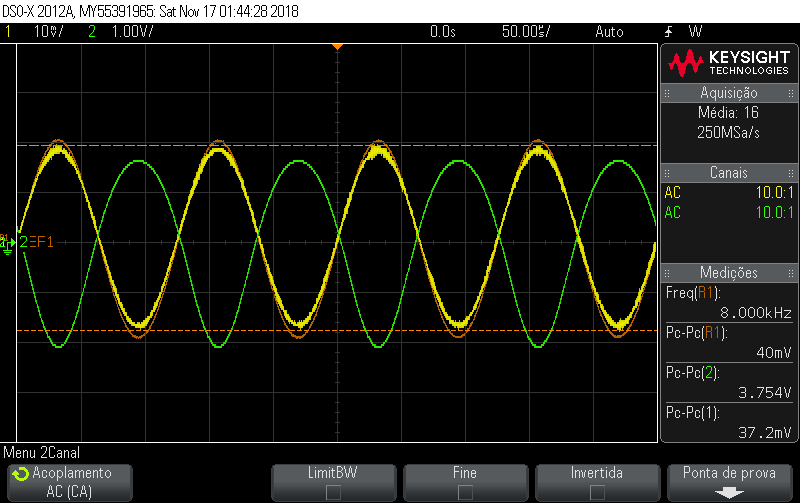
\includegraphics[width=\columnwidth]{osciloscopio_distorcao.png}
    		\caption{Formas de onda de $V_o$ e $V_i$ do circuito da Figura \ref{circuit ideal com distorção} montado no laboratório.}
    		\label{osciloscopio lab com distorção}
    		\end{center}
    	\end{figure}
        
        
\section{Análise dos resultados}
    \tab Ao comparar os resultados obtidos na prática e simulação com os dados calculados previamente, observa-se que, apesar do ganho obtido estar de acordo com o desejado, há uma distorção considerável na saída do Amplificador. Na Figura \ref{osciloscopio lab com distorção}, observa-se a forma de onda da saída distorcida. 
    
    \tab Uma forma mais precisa de observar esse fenômeno se da pela função FFT do Osciloscópio e pode ser observada na Figura \ref{osciloscopio fft}. 
    
         \begin{figure}[H]
    		\begin{center}
    		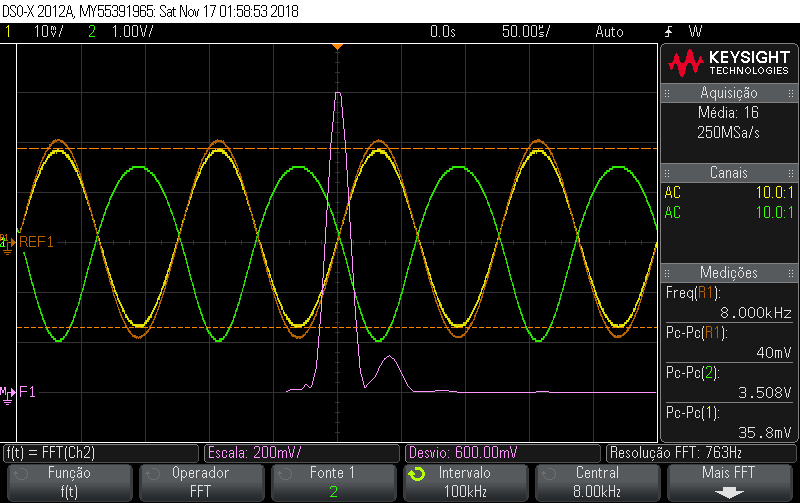
\includegraphics[width=\columnwidth]{osciloscopio_distorcao_fft.png}
    		\caption{Análise FFT do Amplificador.}
    		\label{osciloscopio fft}
    		\end{center}
    	\end{figure}
    
    \tab Em seguida, necessitou-se realizar uma adaptação ao circuito com a finalidade de diminuir a distorção presente. Escolheu-se acrescentar um resistor de degeneração na saída do emissor do transistor, fornecendo uma realimentação negativa que estabiliza a saída. 
    
    \tab Escolhe-se um valor pequeno de $2 \: \Omega$ para tal resistor, de forma a estabilizar a saída, comprometendo o mínimo possível do ganho.
    
    \tab Obesrva-se o circuito a seguir: 
        \begin{figure}[H]
        \hspace{-0.8cm}
        	\begin{tikzpicture}[circuit ee IEC, scale=0.5666666667,line width=.5pt]% default: 0.4
	%\tikzstyle{every node}=[font=\small];%
	%\node [draw] at (0.0,0.0) {\pgfkeysvalueof{/tikz/circuitikz/tripoles/op amp/font}};
%\draw [/lt2ti/Net](22.0,22.5)to[*short,*-, color=netcolor] (22.0,22.5);% wire w3_w6 start
%\draw [/lt2ti/Net](15.5,21.0)to[*short,-, color=netcolor] (15.5,21.0);% wire w3_w6 end
%\draw [/lt2ti/Net](22.0,22.5) --  (15.5,22.5) -- (15.5,21.0); % wire w3_w6 polyline 
\draw [/lt2ti/Net](27.0,22.0)to[*short,-, color=netcolor] (27.0,22.0);% wire w4_w5 start
%\draw [/lt2ti/Net](22.0,22.5)to[*short,-*, color=netcolor] (22.0,22.5);% wire w4_w5 end
%\draw [/lt2ti/Net](27.0,22.0) --  (27.0,22.5) -- (22.0,22.5); % wire w4_w5 polyline 
%\draw [/lt2ti/Net](22.0,21.0)to[*short,-*, color=netcolor] (22.0,22.5);% wire w7
\draw [/lt2ti/Net](27.0,18.5)to[*short,*-, color=netcolor] (27.0,19.1);% wire w8
\draw [/lt2ti/Net](28.0,18.5)to[*short,-*, color=netcolor] (27.0,18.5);% wire w9
%\draw [/lt2ti/Net](15.5,17.5)to[*short,-, color=netcolor] (15.5,18.5);% wire w11
\draw [/lt2ti/Net](31.5,17.5)to[*short,-, color=netcolor] (31.5,17.5);% wire w10_w12 start
\draw [/lt2ti/Net](30.0,18.5)to[*short,-, color=netcolor] (30.0,18.5);% wire w10_w12 end
\draw [/lt2ti/Net](31.5,17.5) --  (31.5,18.5) -- (30.0,18.5); % wire w10_w12 polyline 
\draw [/lt2ti/Net](19.5,17.0)to[*short,-, color=netcolor] (19.5,17.0);% wire w13_w18 start
\draw [/lt2ti/Net](18.0,14.5)to[*short,-, color=netcolor] (18.0,14.5);% wire w13_w18 end
\draw [/lt2ti/Net](19.5,17.0) --  (18.0,17.0) -- (18.0,14.5); % wire w13_w18 polyline 
\draw [/lt2ti/Net](22.0,17.0)to[*short,*-, color=netcolor] (22.0,17.8);% wire w14
\draw [/lt2ti/Net](22.0,17.0)to[*short,*-, color=netcolor] (21.5,17.0);% wire w15
\draw [/lt2ti/Net](25.0,17.0)to[*short,-, color=netcolor] (25.0,17.0);% wire w16_w17 start
\draw [/lt2ti/Net](22.0,17.0)to[*short,-*, color=netcolor] (22.0,17.0);% wire w16_w17 end
\draw [/lt2ti/Net](25.0,17.0) --  (24.0,17.0) -- (22.0,17.0); % wire w16_w17 polyline 
\draw [/lt2ti/Net](22.0,14.5)to[*short,-*, color=netcolor] (22.0,17.0);% wire w19
\draw [/lt2ti/Net](31.5,13.5)to[*short,-, color=netcolor] (31.5,15.0);% wire w20
\draw [/lt2ti/Net](27.0,12.5)to[*short,*-, color=netcolor] (27.0,13.0);% wire w21
\draw [/lt2ti/Net](27.0,12.0)to[*short,-*, color=netcolor] (27.0,12.5);% wire w23
\draw [/lt2ti/Net](29.5,11.5)to[*short,-, color=netcolor] (29.5,11.5);% wire w22_w24 start
\draw [/lt2ti/Net](27.0,12.5)to[*short,-*, color=netcolor] (27.0,12.5);% wire w22_w24 end
\draw [/lt2ti/Net](29.5,11.5) --  (29.5,12.5) -- (27.0,12.5); % wire w22_w24 polyline 
\draw [/lt2ti/Net](22.0,9.0)to[*short,*-, color=netcolor] (22.0,12.0);% wire w26
\draw [/lt2ti/Net](22.0,9.0)to[*short,*-, color=netcolor] (22.0,9.0);% wire w25_w27 start
\draw [/lt2ti/Net](18.0,12.0)to[*short,-, color=netcolor] (18.0,12.0);% wire w25_w27 end
\draw [/lt2ti/Net](22.0,9.0) --  (18.0,9.0) -- (18.0,12.0); % wire w25_w27 polyline 
\draw [/lt2ti/Net](24.0,9.0)to[*short,*-*, color=netcolor] (22.0,9.0);% wire w28
\draw [/lt2ti/Net](27.0,9.0)to[*short,*-, color=netcolor] (27.0,9.5);% wire w29
\draw [/lt2ti/Net](27.0,9.0)to[*short,*-*, color=netcolor] (24.0,9.0);% wire w30
\draw [/lt2ti/Net](29.5,9.5)to[*short,-, color=netcolor] (29.5,9.5);% wire w31_w32 start
\draw [/lt2ti/Net](27.0,9.0)to[*short,-*, color=netcolor] (27.0,9.0);% wire w31_w32 end
\draw [/lt2ti/Net](29.5,9.5) --  (29.5,9.0) -- (27.0,9.0); % wire w31_w32 polyline 
\draw [/lt2ti/Net](24.0,7.5)to[*short,-*, color=netcolor] (24.0,9.0);% wire w33
\draw [/lt2ti/Net](22.0,20.3)to[-*, color=netcolor] (22.0,21.7);% wire teste  

 %\draw (15.5, 17.5) node[ground, xscale=2, yscale=2, rotate=270, ] (undefined) {};%  (undefined)++(0.0,0.0) node {undefined }; % component "circuiTikz\\gnd" "undefined" 
 \draw (24.0, 7.5) node[ground, xscale=2, yscale=2, rotate=270, ] (undefined) {};%  (undefined)++(0.0,0.0) node {undefined }; % component "circuiTikz\\gnd" "undefined" 
 \draw (31.5, 13.5) node[ground, xscale=2, yscale=2, rotate=270, ] (undefined) {};%  (undefined)++(0.0,0.0) node {undefined }; % component "circuiTikz\\gnd" "undefined" 
  \draw (22.0, 20.3) to[*resistor, l^=R\textsubscript{1},  -, ] (22.0,17.8){}; %\node [] at (21.5,21.5) {x}; % component "res" "R9" 
  \draw  --++(22,21.6) node[vcc]{+\,\textnormal{V\textsubscript{CC}}}{};% to (22,20.3){};
  \draw (22.0, 14.5) to[*resistor, l^=R\textsubscript{2}, , -, ] (22.0,12.0){}; %\node [] at (21.5,15.0) {x}; % component "res" "R10" 
  \draw (27.0, 21.6) to[*resistor, l^=R\textsubscript{C},  -, ] (27.0,19.1){}; %\node [] at (26.5,22.5) {x}; % component "res" "R11" 
  \draw  --++(27,21.7) node[vcc]{+\,\textnormal{V\textsubscript{CC}}} to (27,21.6){};
  \draw (27.0, 12.0) to[*resistor, a_=R\textsubscript{E},  -, ] (27.0,9.5){}; %\node [] at (26.5,12.5) {x}; % component "res" "R12" 
 \draw (27.0, 17.0) node[npn, nobodydiode, , rotate=0, ] (Q3) {}  ; % component "npn" "Q3" 
 \draw (25.0, 17.0) to [*short, -] (Q3.B); \draw (27.0, 15.5) to [*short, -] (Q3.E); \draw (27.0, 18.5) to [*short, -] (Q3.C);% extend wires to the connection points   % component "npn" "Q3" 
%  \draw (15.5, 21.0) to[*V, l_=V\textsubscript{CC}, , -, ] (15.5,18.5){}; % component "voltage" "V5" 
  \draw (21.5, 17.0) to[*capacitor, l^=C,  -, ] (19.5,17.0){}; % component "cap" "C5" 
  %\node [] at (21.5,17.5) {x}; % component "cap" "C5" 
  \draw (30.0, 18.5) to[*capacitor, l^=C, -, ] (28.0,18.5){}; % component "cap" "C6" 
  %\node [] at (30.0,19.0) {x}; % component "cap" "C6" 
  \draw (18.0, 14.5) to[*V, l_=V\textsubscript{sig}, , -, ] (18.0,12.0){}; % component "voltage" "V3" 
  \draw (29.5, 11.5) to[*capacitor, l^=C,  -, ] (29.5,9.5){}; % component "cap" "C3" 
  %\node [] at (29.0,11.5) {x}; % component "cap" "C3" 
  \draw (31.5, 17.5) to[*resistor, l^=R\textsubscript{L},  -, ] (31.5,15.0){}; %\node [] at (31.0,18.0) {x}; % component "res" "R6" 
  \draw (27.0, 15.5) to[*resistor,  a_=2 $\Omega$,l^=R\textsubscript{e}, -, ] (27.0,13.0){}; %\node [] at (26.5,16.0) {x}; % component "res" "R7" 
  \node (Vo) [] at (31.5,18.5) {};% label mark % label "" "Vo" lbl37 
%  \node (Votxt) [ netlabelcolor, above= -0.24cm of Vo] {{\pgfkeysvalueof{/lt2ti/netlabel/font}Vo}}; % label "" "Vo" lbl37 
  \node (Vi) [] at (24.0,17.0) {};% label mark % label "" "Vi" lbl38 
%  \node (Vitxt) [ netlabelcolor, above= -0.24cm of Vi] {{\pgfkeysvalueof{/lt2ti/netlabel/font}Vi}}; % label "" "Vi" lbl38 
  \node (Vsig) [] at (18.0,17.0) {};% label mark % label "" "Vsig" lbl39 
%  \node (Vsigtxt) [ netlabelcolor, above= -0.24cm of Vsig] {{\pgfkeysvalueof{/lt2ti/netlabel/font}Vsig}}; % label "" "Vsig" lbl39 
  \node (lbl86) [] at (17.0,7.75) {};% text mark % text "" ".tran 1ms lbl86 " 
%  \node (lbl86txt) [ lttotitextcolor, right= -0.25cm of lbl86, scale=0.5*2.0] {{\pgfkeysvalueof{/lt2ti/text/font}.tran 1ms}}; % text "" ".tran 1ms lbl86 " 

	\end{tikzpicture}
	
	
	
	
	
	
	
	
	
	
	
	
	
	
	
	
	
	
	
	
	
	
	
	
	
	
	
	
	
	
	
	
	
	
	
	
	
	
	
	
	
	
	
	
	
	
	
	
	
	
	
	
	
	
	
	
	
	
	
	
	
	
	
	
	
	
	
	
	
	
	
	
	
	
	
	
	
	
	
	
	
	
	
	
	
	
	
	
	
	
	
	
	
	
	
	
	
	
	
	
	
	
	

%%%%%%%%%%%%%%%%%%%%%%%%%%%%%%%%%%%%%%%%%%%%%%%%%%%%%%%%%%%%%%%%%%%%%%%%%%%%%%%%%%%%%%%%%%%%%%%%%%%%%%%%%% VERSÃO ANTIGA %%%%%%%%%%%%%%%%%%%%%%%%%%%%%%%%%%% %%%%%%%%%%%%%%%%%%%%%%%%%%%%%%%%%%%%%%%%%%%%%%%%%%%%%%%%%%%%%%%%%%%%%%%%%%%%%%
% automatically generated document using lt2circuiTikz

%\usepackage{agaramondc}					% Adobe Garamond, custom shape
%\renewcommand{\shapedefault}{rtl} % rtl: roman tabular lining

%\makeatletter

%% bandstop filter (adapted from highpass)
\pgfcircdeclarebipole{}{\ctikzvalof{bipoles/highpass/width}}{*bandstop}{\ctikzvalof{bipoles/highpass/width}}{\ctikzvalof{bipoles/highpass/width}}{
	\pgf@circ@res@step = \ctikzvalof{bipoles/highpass/width}\pgf@circ@Rlen
	\divide \pgf@circ@res@step by 2
	
	\pgfpathmoveto{\pgfpoint{\pgf@circ@res@left}{\pgf@circ@res@zero}}
	\pgf@circ@res@other = \pgf@circ@res@left
	\advance\pgf@circ@res@other by \pgf@circ@res@step 
	
	\ifpgf@circuit@dashed
	\pgfsetdash{{0.1cm}{0.1cm}}{0cm} 
	\fi	
	
	% draw outer box
	\pgfsetlinewidth{\pgfkeysvalueof{/tikz/circuitikz/bipoles/thickness}\pgfstartlinewidth}
	\pgfpathrectanglecorners{\pgfpoint{\pgf@circ@res@left}{\pgf@circ@res@up}}{\pgfpoint{\pgf@circ@res@right}{\pgf@circ@res@down}}
	\pgfusepath{draw}
	
	\ifpgf@circuit@inputarrow
	{
		\advance \pgf@circ@res@left by -.5\pgfkeysvalueof{/tikz/circuitikz/bipoles/thickness}\pgfstartlinewidth
		\pgftransformshift{\pgfpoint{\pgf@circ@res@left}{0pt}}
		\pgfnode{inputarrow}{tip}{}{pgf@inputarrow}{\pgfusepath{fill}}
	}
	\fi
	
	% rotate inner symbol
	\def\pgfcircmathresult{\expandafter\pgf@circ@stripdecimals\pgf@circ@direction\pgf@nil}
	\ifnum \pgfcircmathresult > 45 \ifnum \pgfcircmathresult < 135
	\pgftransformrotate{270}
	\fi\fi
	\ifnum \pgfcircmathresult > 134 \ifnum \pgfcircmathresult < 225  % 134 degree, because >= 135 is not possible
	\pgftransformrotate{180}
	\fi\fi
	\ifnum \pgfcircmathresult > 224 \ifnum \pgfcircmathresult < 315
	\pgftransformrotate{90}
	\fi\fi
	
	% draw inner symbol
	\pgfsetdash{}{0pt}	% always draw solid line for inner symbol
	\pgfsetarrows{-} %never draw arrows
	\pgfsetlinewidth{\pgfstartlinewidth}
	\pgfpathmoveto{\pgfpoint{-0.5\pgf@circ@res@step}{0.5\pgf@circ@res@step}}
	\pgfpathsine{\pgfpoint{.25\pgf@circ@res@step}{.25\pgf@circ@res@step}}
	\pgfpathcosine{\pgfpoint{.25\pgf@circ@res@step}{-.25\pgf@circ@res@step}}
	\pgfpathsine{\pgfpoint{.25\pgf@circ@res@step}{-.25\pgf@circ@res@step}}
	\pgfpathcosine{\pgfpoint{.25\pgf@circ@res@step}{.25\pgf@circ@res@step}}
	\pgfusepath{draw}
	
	\pgfpathmoveto{\pgfpoint{-0.5\pgf@circ@res@step}{0}}
	\pgfpathsine{\pgfpoint{.25\pgf@circ@res@step}{.25\pgf@circ@res@step}}
	\pgfpathcosine{\pgfpoint{.25\pgf@circ@res@step}{-.25\pgf@circ@res@step}}
	\pgfpathsine{\pgfpoint{.25\pgf@circ@res@step}{-.25\pgf@circ@res@step}}
	\pgfpathcosine{\pgfpoint{.25\pgf@circ@res@step}{.25\pgf@circ@res@step}}
	\pgfusepath{draw}
	\pgfpathmoveto{\pgfpoint{-0.15\pgf@circ@res@step}{-0.15\pgf@circ@res@step}}
	\pgfpathlineto{\pgfpoint{0.15\pgf@circ@res@step}{0.15\pgf@circ@res@step}}
	\pgfusepath{draw}
	
	\pgfpathmoveto{\pgfpoint{-0.5\pgf@circ@res@step}{-0.5\pgf@circ@res@step}}
	\pgfpathsine{\pgfpoint{.25\pgf@circ@res@step}{.25\pgf@circ@res@step}}
	\pgfpathcosine{\pgfpoint{.25\pgf@circ@res@step}{-.25\pgf@circ@res@step}}
	\pgfpathsine{\pgfpoint{.25\pgf@circ@res@step}{-.25\pgf@circ@res@step}}
	\pgfpathcosine{\pgfpoint{.25\pgf@circ@res@step}{.25\pgf@circ@res@step}}
	\pgfusepath{draw}
	%	\pgfpathmoveto{\pgfpoint{-0.15\pgf@circ@res@step}{-0.65\pgf@circ@res@step}}
	%	\pgfpathlineto{\pgfpoint{0.15\pgf@circ@res@step}{-0.35\pgf@circ@res@step}}
	%	\pgfusepath{draw}
}

\tikzset{
	*bandstop/.style={\circuitikzbasekey, /tikz/to path=\pgf@circ@*bandstop@path},
}
\def\pgf@circ@*bandstop@path#1{\pgf@circ@bipole@path{*bandstop}{#1}}




\makeatother

% sym32a style

\begin{comment}
%\begin{document}%
	%\centering%
			\begin{tikzpicture}[circuit ee IEC, scale=0.4666666667,line width=.5pt]
            		% default: 0.4
            	%\tikzstyle{every node}=[font=\small];%
            	%\node [draw] at (0.0,0.0) {\pgfkeysvalueof{/tikz/circuitikz/tripoles/op amp/font}};
            \draw [/lt2ti/Net](22.0,22.5)to[*short,*-, color=netcolor] (22.0,22.5);% wire w3_w6 start
            \draw [/lt2ti/Net](15.5,21.0)to[*short,-, color=netcolor] (15.5,21.0);% wire w3_w6 end
            \draw [/lt2ti/Net](22.0,22.5) --  (15.5,22.5) -- (15.5,21.0); % wire w3_w6 polyline 
            \draw [/lt2ti/Net](27.0,22.0)to[*short,-, color=netcolor] (27.0,22.0);% wire w4_w5 start
            \draw [/lt2ti/Net](22.0,22.5)to[*short,-*, color=netcolor] (22.0,22.5);% wire w4_w5 end
            \draw [/lt2ti/Net](27.0,22.0) --  (27.0,22.5) -- (22.0,22.5); % wire w4_w5 polyline 
            \draw [/lt2ti/Net](22.0,21.0)to[*short,-*, color=netcolor] (22.0,22.5);% wire w7
            \draw [/lt2ti/Net](27.0,18.5)to[*short,*-, color=netcolor] (27.0,19.5);% wire w8
            \draw [/lt2ti/Net](28.0,18.5)to[*short,-*, color=netcolor] (27.0,18.5);% wire w9
            \draw [/lt2ti/Net](15.5,17.5)to[*short,-, color=netcolor] (15.5,18.5);% wire w11
            \draw [/lt2ti/Net](31.5,17.5)to[*short,-, color=netcolor] (31.5,17.5);% wire w10_w12 start
            \draw [/lt2ti/Net](30.0,18.5)to[*short,-, color=netcolor] (30.0,18.5);% wire w10_w12 end
            \draw [/lt2ti/Net](31.5,17.5) --  (31.5,18.5) -- (30.0,18.5); % wire w10_w12 polyline 
            \draw [/lt2ti/Net](19.5,17.0)to[*short,-, color=netcolor] (19.5,17.0);% wire w13_w18 start
            \draw [/lt2ti/Net](18.0,14.5)to[*short,-, color=netcolor] (18.0,14.5);% wire w13_w18 end
            \draw [/lt2ti/Net](19.5,17.0) --  (18.0,17.0) -- (18.0,14.5); % wire w13_w18 polyline 
            \draw [/lt2ti/Net](22.0,17.0)to[*short,*-, color=netcolor] (22.0,18.5);% wire w14
            \draw [/lt2ti/Net](22.0,17.0)to[*short,*-, color=netcolor] (21.5,17.0);% wire w15
            \draw [/lt2ti/Net](25.0,17.0)to[*short,-, color=netcolor] (25.0,17.0);% wire w16_w17 start
            \draw [/lt2ti/Net](22.0,17.0)to[*short,-*, color=netcolor] (22.0,17.0);% wire w16_w17 end
            \draw [/lt2ti/Net](25.0,17.0) --  (24.0,17.0) -- (22.0,17.0); % wire w16_w17 polyline 
            \draw [/lt2ti/Net](22.0,14.5)to[*short,-*, color=netcolor] (22.0,17.0);% wire w19
            \draw [/lt2ti/Net](31.5,13.5)to[*short,-, color=netcolor] (31.5,15.0);% wire w20
            \draw [/lt2ti/Net](27.0,12.5)to[*short,*-, color=netcolor] (27.0,13.0);% wire w21
            \draw [/lt2ti/Net](27.0,12.0)to[*short,-*, color=netcolor] (27.0,12.5);% wire w23
            \draw [/lt2ti/Net](29.5,11.5)to[*short,-, color=netcolor] (29.5,11.5);% wire w22_w24 start
            \draw [/lt2ti/Net](27.0,12.5)to[*short,-*, color=netcolor] (27.0,12.5);% wire w22_w24 end
            \draw [/lt2ti/Net](29.5,11.5) --  (29.5,12.5) -- (27.0,12.5); % wire w22_w24 polyline 
            \draw [/lt2ti/Net](22.0,9.0)to[*short,*-, color=netcolor] (22.0,12.0);% wire w26
            \draw [/lt2ti/Net](22,21.7)to[*short,*-, %color=netcolor] (22,20.3);% wire teste
            \draw [/lt2ti/Net](22.0,9.0)to[*short,*-, color=netcolor] (22.0,9.0);% wire w25_w27 start
            \draw [/lt2ti/Net](18.0,12.0)to[*short,-, color=netcolor] (18.0,12.0);% wire w25_w27 end
            \draw [/lt2ti/Net](22.0,9.0) --  (18.0,9.0) -- (18.0,12.0); % wire w25_w27 polyline 
            \draw [/lt2ti/Net](24.0,9.0)to[*short,*-*, color=netcolor] (22.0,9.0);% wire w28
            \draw [/lt2ti/Net](27.0,9.0)to[*short,*-, color=netcolor] (27.0,9.5);% wire w29
            \draw [/lt2ti/Net](27.0,9.0)to[*short,*-*, color=netcolor] (24.0,9.0);% wire w30
            \draw [/lt2ti/Net](29.5,9.5)to[*short,-, color=netcolor] (29.5,9.5);% wire w31_w32 start
            \draw [/lt2ti/Net](27.0,9.0)to[*short,-*, color=netcolor] (27.0,9.0);% wire w31_w32 end
            \draw [/lt2ti/Net](29.5,9.5) --  (29.5,9.0) -- (27.0,9.0); % wire w31_w32 polyline 
            \draw [/lt2ti/Net](24.0,7.5)to[*short,-*, color=netcolor] (24.0,9.0);% wire w33
             \draw (15.5, 17.5) node[ground, xscale=2, yscale=2, rotate=270, ] (undefined) {};%  (undefined)++(0.0,0.0) node {undefined }; % component "circuiTikz\\gnd" "undefined" 
             \draw (24.0, 7.5) node[ground, xscale=2, yscale=2, rotate=270, ] (undefined) {};%  (undefined)++(0.0,0.0) node {undefined }; % component "circuiTikz\\gnd" "undefined" 
             \draw (31.5, 13.5) node[ground, xscale=2, yscale=2, rotate=270, ] (undefined) {};%  (undefined)++(0.0,0.0) node {undefined }; % component "circuiTikz\\gnd" "undefined" 
              \draw (22.0, 21.0) to[*resistor, l^=R\textsubscript{1},  -, ] (22.0,18.5){}; %\node [] at (21.5,21.5) {x}; % component "res" "R9" 
              \draw (22.0, 14.5) to[*resistor, l^=R\textsubscript{2}, , -, ] (22.0,12.0){}; %\node [] at (21.5,15.0) {x}; % component "res" "R10" 
              \draw (27.0, 22.0) to[*resistor, l^=R\textsubscript{C},  -, ] (27.0,19.5){}; %\node [] at (26.5,22.5) {x}; % component "res" "R11" 
              \draw (27.0, 12.0) to[*resistor, a_=R\textsubscript{E},   -, ] (27.0,9.5){}; %\node [] at (26.5,12.5) {x}; % component "res" "R12" 
             \draw (27.0, 17.0) node[npn, nobodydiode, , rotate=0, ] (Q3) {}  ; % component "npn" "Q3" 
             \draw (25.0, 17.0) to [*short, -] (Q3.B); \draw (27.0, 15.5) to [*short, -] (Q3.E); \draw (27.0, 18.5) to [*short, -] (Q3.C);% extend wires to the connection points   % component "npn" "Q3" 
              \draw (15.5, 21.0) to[*V, l_=V\textsubscript{CC}, , -, ] (15.5,18.5){}; % component "voltage" "V5" 
              \draw (21.5, 17.0) to[*capacitor, l^=C,  -, ] (19.5,17.0){}; % component "cap" "C5" 
              %\node [] at (21.5,17.5) {x}; % component "cap" "C5" 
              \draw (30.0, 18.5) to[*capacitor, l^=C, -, ] (28.0,18.5){}; % component "cap" "C6" 
              %\node [] at (30.0,19.0) {x}; % component "cap" "C6" 
              \draw (18.0, 14.5) to[*V, l_=V\textsubscript{sig}, , -, ] (18.0,12.0){}; % component "voltage" "V3" 
              \draw (29.5, 11.5) to[*capacitor, l^=C,  -, ] (29.5,9.5){}; % component "cap" "C3" 
              %\node [] at (29.0,11.5) {x}; % component "cap" "C3" 
              \draw (31.5, 17.5) to[*resistor, l^=R\textsubscript{L},  -, ] (31.5,15.0){}; %\node [] at (31.0,18.0) {x}; % component "res" "R6" 
              \draw (27.0, 15.5) to[*resistor,  a_=2 $\Omega$, l^=R\textsubscript{e}, -, ] (27.0,13.0){}; %\node [] at (26.5,16.0) {x}; % component "res" "R7" 
              \node (Vo) [] at (31.5,18.5) {};% label mark % label "" "Vo" lbl37 
            %  \node (Votxt) [ netlabelcolor, above= -0.24cm of Vo] {{\pgfkeysvalueof{/lt2ti/netlabel/font}Vo}}; % label "" "Vo" lbl37 
              \node (Vi) [] at (24.0,17.0) {};% label mark % label "" "Vi" lbl38 
            %  \node (Vitxt) [ netlabelcolor, above= -0.24cm of Vi] {{\pgfkeysvalueof{/lt2ti/netlabel/font}Vi}}; % label "" "Vi" lbl38 
              \node (Vsig) [] at (18.0,17.0) {};% label mark % label "" "Vsig" lbl39 
            %  \node (Vsigtxt) [ netlabelcolor, above= -0.24cm of Vsig] {{\pgfkeysvalueof{/lt2ti/netlabel/font}Vsig}}; % label "" "Vsig" lbl39 
              \node (lbl86) [] at (17.0,7.75) {};% text mark % text "" ".tran 1ms lbl86 " 
            %  \node (lbl86txt) [ lttotitextcolor, right= -0.25cm of lbl86, scale=0.5*2.0] {{\pgfkeysvalueof{/lt2ti/text/font}.tran 1ms}}; % text "" ".tran 1ms lbl86 " \
    
    	\end{tikzpicture}
%\end{document}
\end{comment}
        
	    \caption{Amplificador Emissor-Comum com resistor de degeneração.}
        \label{EM com re}
    \end{figure}
    
    \tab Ainda assim, o acréscimo de R\textsubscript{e} causou uma redução no ganho $A_v$, precisando, assim, ajustar certos parâmetros do projeto do Amplificador para manter o ganho $A_v$ igual à $-100 \:$ V/V.
    
    \tab Escolheu-se manter os valores dos Resistores e ajustar a alimentação $V_{CC}$.
    
    \tab Deste modo, calcula-se: 
    
     \tab A partir da análise c.a dos amplificador, usando o modelo T, tem-se que:
     
       $$     A_v = \frac{-\alpha(R_C//R_L)}{r_e + R_e} = -100 $$
      
    \tab Assim, 
     
       $$     r_e+2 = \frac{\alpha(R_C//R_L)}{100} = 4,95$$
       
       $$ r_e =2,95 = \frac{0,025}{I_E} \Rightarrow I_E = \SI{8,4745}{\milli\ampere}$$
       
       $$I_B = \frac{I_E}{\beta+1} = \SI{83,9}{\micro\ampere}$$
       
    \tab Em que,  
       $$ I_B = \frac{V_{TH}-V_{BE}}{R_{TH}+(\beta+1)R_{E}} \Rightarrow \: V_{TH} = \SI{2,627}{\volt}$$
       
    \tab Além disso,
      $$ V_{TH}= \frac{R_2 \times V_{CC} }{R_2+R_1} \Rightarrow \: V_{CC} = \frac{V_{TH} \times(R_2+R_1) }{R_2} = \SI{14,3}{\volt}.$$
     \vspace{0.3 cm} 
      
    \tab Nas Figuras \ref{osciloscopio com menor distorção} e \ref{fft com re} observa-se a simulação e a análise FFT do novo circuito, respectivamente. 
        
        \begin{figure}[H]
    		\begin{center}
    		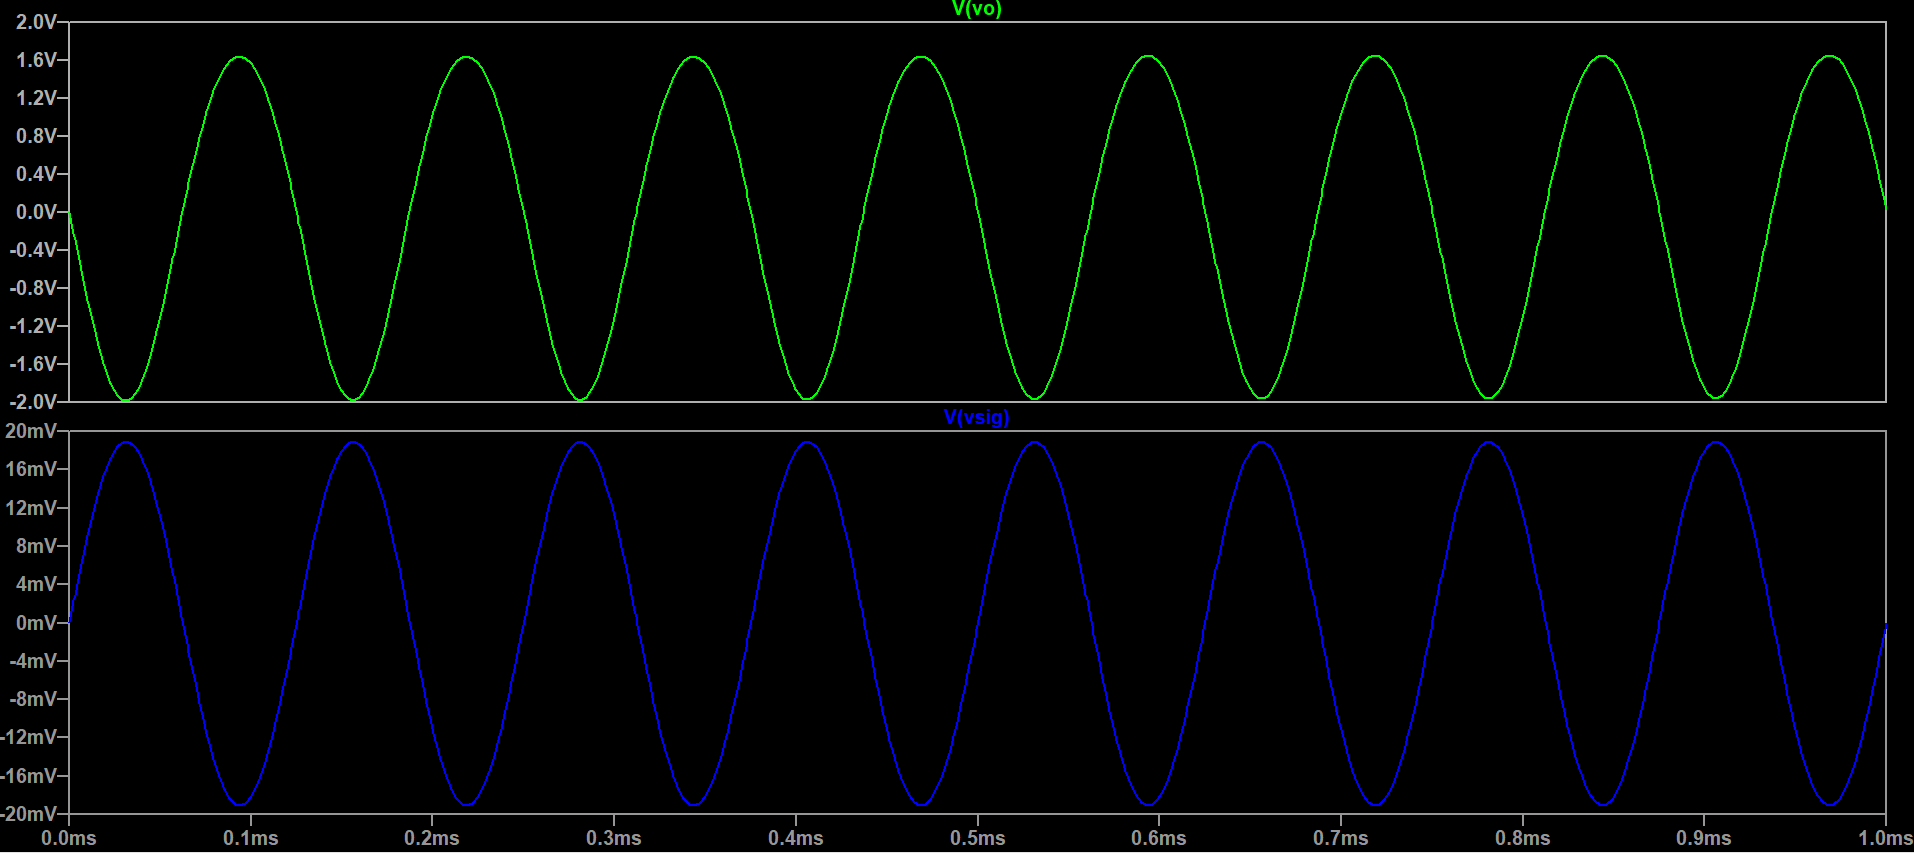
\includegraphics[width=\columnwidth]{Av_menor_distorcao.PNG}
    		\caption{Formas de onda de $V_o$ e $V_i$ do circuito da Figura \ref{EM com re}.}
    		\label{osciloscopio com menor distorção}
    		\end{center}
    	\end{figure}
    	
    	\begin{figure}[H]
    		\begin{center}
    		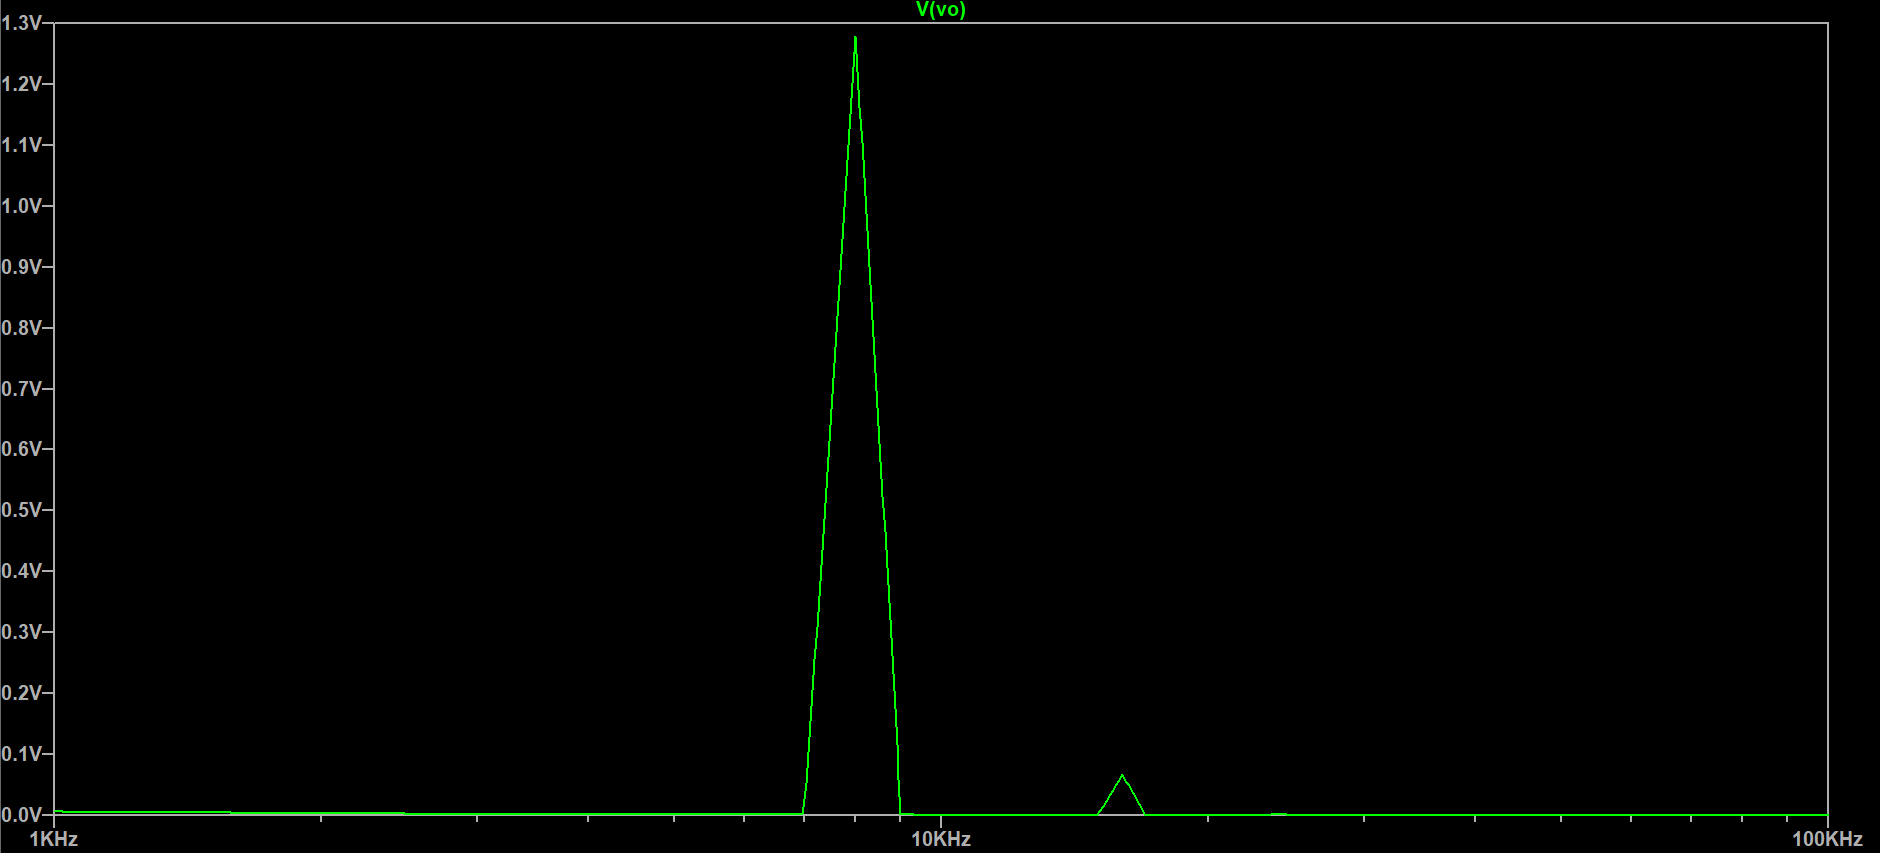
\includegraphics[width=\columnwidth]{fft_com_re.PNG}
    		\caption{Análise FFT do Amplificador da Figura \ref{EM com re}.}
    		\label{fft com re}
    		\end{center}
    	\end{figure}
    	
    \tab Finalmente, com o auxílio da ferramenta \textit{Cursor}, verificou-se o valor da magnitude do segundo pico da FFT como 66,9 mV. O que representa uma redução considerável de distorção. Visto que, antes do acréscimo de $R_e$, o valor da magnitude do segundo pico da FFT era igual à 199,23 mV.
        
\end{document}